\section{Моделирование нейронных сетей и алгоритмов обучения}

\subsection{Моделирование нейронной сети}

Для распознавания цифр спроектирована нейронная сеть состоящая из трех слоев.

На входном слое $28 * 28 = 784$ нейрона, да ещё и нейрон смещения (bias). Итого $785$.

Скрытый слой только один, состоящий из 128 нейронов. Срытый слоев может быть несколько, хоть и два и три. Нейронов в срытом слое может быть разное количество, хоть и 50 нейронов.

На выходном слое у нас 10 нейронов, то есть 10 классов: ноль, один, два, три, четыре, пять, шесть, семь, восемь, девять.

Спроектированная нейронная сеть на
рисунке~\textbf{\ref{fig:3_NNDiagram} (стр. \pageref{fig:3_NNDiagram})}.

\begin{figure}[p]
    \centering
    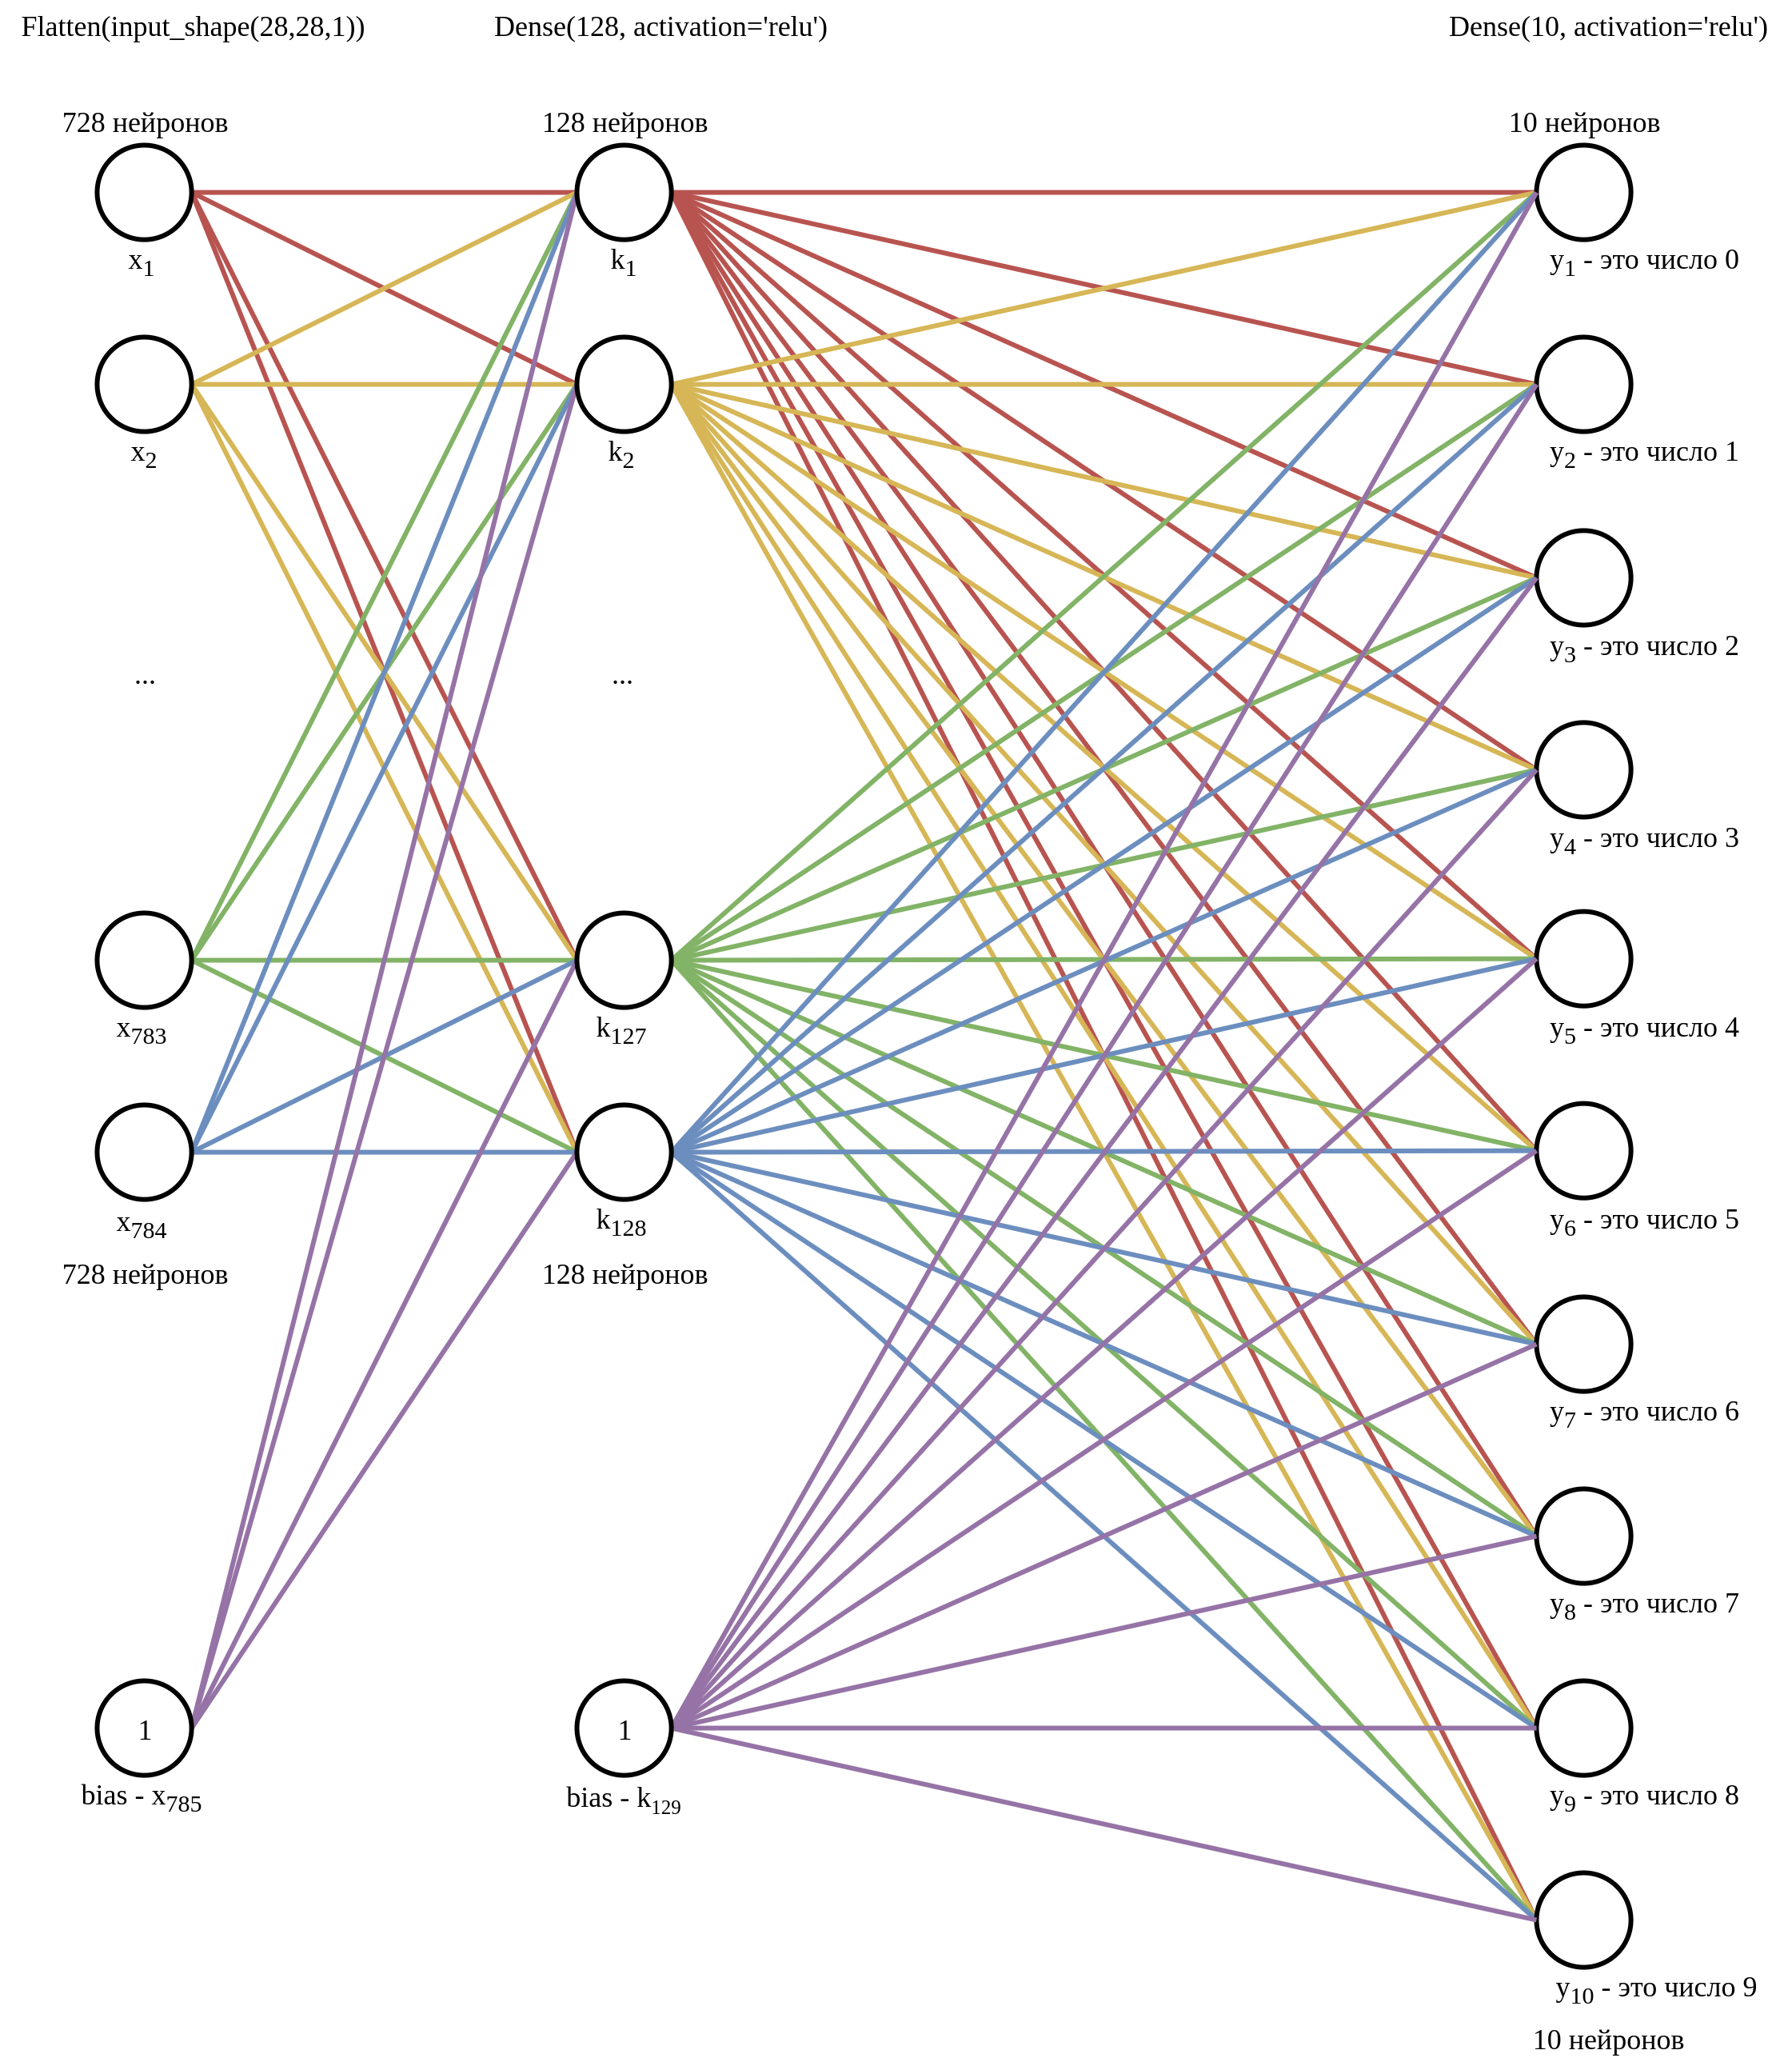
\includegraphics[width=16cm]
    {../../src/digits/NNDiagram.png}
    \caption{Схема нейронной сети}
    \label{fig:3_NNDiagram}
\end{figure}

На вход будем подавать изображения с БД MNIST.

\begin{lstlisting}[language=Python,]
    (x_train, y_train), (x_test, y_test) = tensorflow.keras.datasets.mnist.load_data()
\end{lstlisting}

Где <<\verb|x_train|>> - изображения цифр обучающей выборки.

Где <<\verb|у_train|>> - вектор соответсвующих значений цифр,
если на i-отом изображении нарисовано 5, то \verb|y_train[i] = 5|.

Где <<\verb|x_test|>> - изображения цифр тестовой выборки.

Где <<\verb|у_test|>> - вектор соответствующих значений цифр для тестовой выборки,
если на i-отом изображении нарисовано 5, то \verb|y_test[i] = 5|.

Для подачи значений на входной слой значения нужно нормировать поделив на 255, где 255 - максимальное число, то есть при делении получим значение от нуля до единицы.

\begin{lstlisting}[language=Python,]
    # стандартизация входных данных
    x_train = x_train / 255
    x_test = x_test / 255
\end{lstlisting}

Моделируем сеть библиотекой Keras.

\begin{lstlisting}[language=Python,]
    model = tensorflow.keras.Sequential([
        tensorflow.keras.layers.Flatten(input_shape=(28, 28, 1)),
        tensorflow.keras.layers.Dense(128, activation='relu'),
        tensorflow.keras.layers.Dense(10, activation='softmax')  ])
\end{lstlisting}

\newpage

\subsection{Функция активации}

В искусственных нейронных сетях функция активации нейрона определяет выходной сигнал,
который определяется входным сигналом или набором входных сигналов.

В нашей сети функции активации имеют скрытый и выходной слой.
Скрытый слой имеет функцию активации ReLu.
Выходной слой имеет функцию активации softmax.

\subsubsection{ReLu}

ReLu - функция активации, которая позволяет решать не линейные задачи.

ReLu имеет формулу вида $y_i = max(0, x_i)$,
для i-того нейрона.

График функции изображен на
рисунке~\textbf{\ref{fig:3_ReLu} (стр. \pageref{fig:3_ReLu})}.

\begin{figure}[!htp]
    \centering
    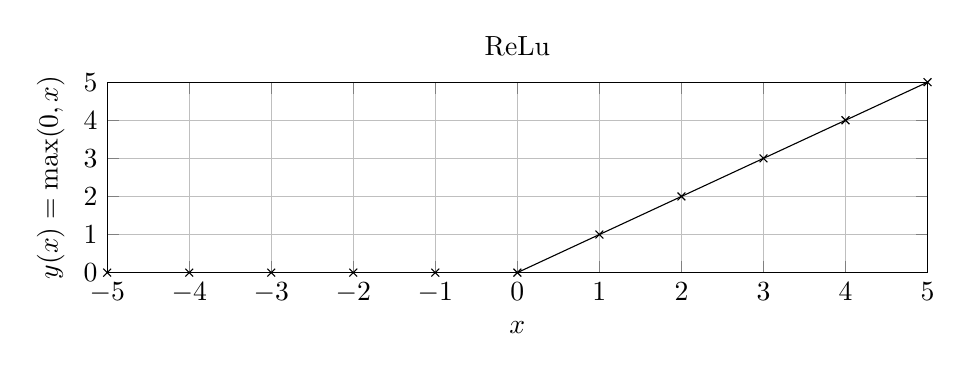
\begin{tikzpicture}
        \begin{axis}[
            title=ReLu,
            width=12cm,
            height=4cm,
            grid,
            %
            xtick distance=1,
            xmin=-5,
            xmax=5,
            xlabel={$x$},
            %
            ytick distance=1,
            ymin=0,
            ymax=5,
            ylabel=${y(x) = \max(0, x)}$,
        ]
            \addplot[color=black, mark=x] coordinates {
                (-5,  0)
                (-4, 0)
                (-3, 0)
                (-2, 0)
                (-1, 0)
                (0, 0)
                (1, 1)
                (2, 2)
                (3, 3)
                (4, 4)
                (5, 5)
            };
        \end{axis}
    \end{tikzpicture}
    \caption{ReLu}
    \label{fig:3_ReLu}
\end{figure}

\subsubsection{Softmax}

Softmax - функция активации, которая вычисляет вероятность для каждого возможного выходного класса.

Softmax имеет формулу вида $y_i = { e^{x_i} \over \sum\limits_{j=1}^n e^{x_i} }$,
для i-того нейрона.
